\documentclass{article}
\usepackage{graphicx}
\usepackage[utf8]{inputenc}
\usepackage[T1]{fontenc}
\usepackage{imakeidx}
\usepackage{hyperref}
\makeindex

\title{Git for Robots}   
\author{Arjun Gandhi} 
\date{\today} 

\begin{document}


%=========================================
\begin{titlepage}
		\centering{
			{\fontsize{40}{48}\selectfont 
			Git for Robotics}
		}\\
			
		\vspace{10mm}
		\centering{\Large{Arjun Gandhi}}\\
		\vspace{\fill}
		\centering \large{March 2020}
\end{titlepage}


%=========================================
\newpage{}
\thispagestyle {empty}

\vspace*{2cm}

\begin{figure}
		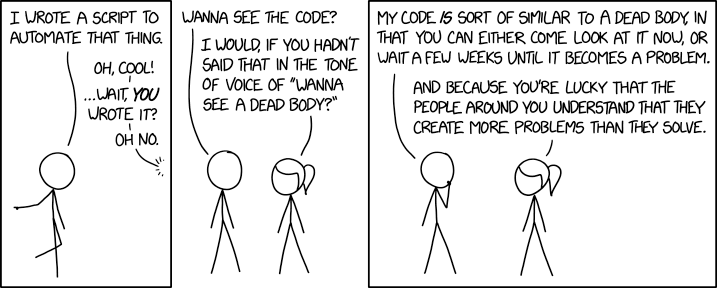
\includegraphics[width=5.5in]{images/wanna_see_the_code.png}
		\caption{This is how all of my robotics project go.}
\end{figure}

\newpage

\tableofcontents

\newpage
\section{What is version control?}
\paragraph{}
    You can think of a version control system (short: "VCS\index{version control system}") as a kind of "database". It lets you save a snapshot of your complete project at any time you want. When you later take a look at an older snapshot (let's start calling it "version\index{version}"), your VCS shows you exactly how it differed from the previous one.
    \begin{figure}[hp]
    \centering
    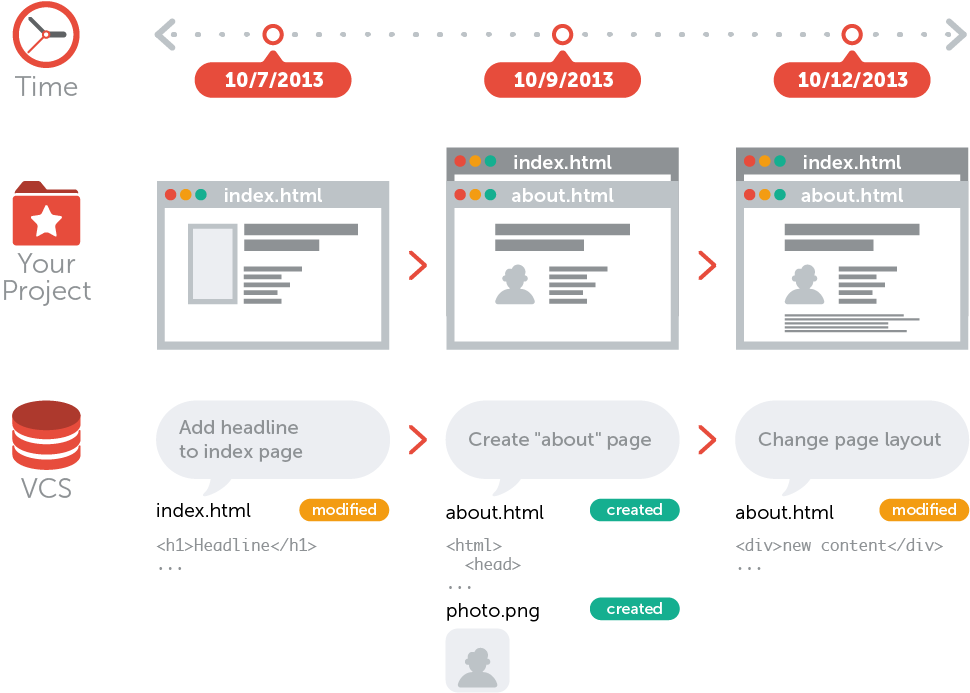
\includegraphics[width=4.5in]{images/what_is_vcs.png}
    \end{figure}
    
    Version control is independent of the kind of project / technology / framework you're working with:
    \begin{itemize}
        \item It works a website as it does for a robotics project
        \item It lets you work with any tool you like; it doesn't care what kind of text editor, graphics program, file manager or other tool you use
    \end{itemize}

    At the core of it a VCS records the changes you make to your project's files. This is what version control is about. It's really as simple as it sounds.
\subsection{Why use version control}
    \paragraph{}
    With out a VCS you are probably working together in a shared folder on the same set of files. Texting your teammates that you are currently working on file "xyz" and that, meanwhile, your teammates should keep their fingers off. This is an awful idea. It's extremely error-prone as you're essentially doing open-heart surgery all the time: sooner or later, someone will overwrite someone else's changes.

    With a VCS, everybody on the team is able to work absolutely freely - on any file at any time. The VCS will later allow you to merge all the changes into a common version. There's no question where the latest version of a file or the whole project is. It's in a common, central place: your version control system.

    Other benefits of using a VCS are even independent of working in a team or on your own.
    
    \subsubsection{Storing Versions (Properly)}
    Making a save of your project after you make critical changes is an important and necessary habit. It prevents you from losing your new work and allows you to go back to your old work easily in case you need it. Without a VCS your save system might look like the following awful ideas (I have personally seen someone do every one of these).
    \begin{itemize}
        \item Saving the changes as a new file and appending a number/date to the end.
        \item Making a copy of the entire code and pasting it (commented out) below the actual code for each versiion of the code.
        %add more fun bad examples if you can think of it
    \end{itemize}
    The core of this however is that the problem gets out of hand fast. 
    
    A VCS solves this problem. A version control system acknowledges that there is only one project. Therefore, there's only the one version on your disk that you're currently working on. Everything else - all the past versions and variants - are neatly packed up inside the VCS. When you need it, you can request any version at any time and you'll have a snapshot of the complete project right at hand.
    \subsubsection{Restoring Old Versions}
    Being able to restore older versions of a file (or even the whole project) effectively means one thing: you can't mess up! If the changes you've made lately prove to be garbage, you can simply undo them in a few clicks. Knowing this should make you a lot more relaxed when working on important bits of a project.
    
    \subsubsection{Understanding What Changes Were Made}
    When working in large teams understanding what changes other members have done quickly is crucial to efficient working. 
    
    Every time you save a new version of your project, your VCS requires you to provide a short description of what was changed. Additionally (if it's a code / text file), you can see what exactly was changed in the file's content. This helps you understand how your project evolved between versions.
    
    \subsubsection{Backup}
    It's happened to all of us before you accidental deleted a critical file in a moment of panic. Luckily a side-effect of using a distributed VCS like Git is that it can act as a backup; every team member has a full-blown version of the project on his disk - including the project's complete history. Should your beloved central server break down (and your backup drives fail), all you need for recovery is one of your teammates' local Git repository.
    
    \subsubsection{What is Git?}
    By far, the most widely used modern version control system in the world today is Git. Git is a mature, actively maintained open source project originally developed in 2005 by Linus Torvalds, the famous creator of the Linux operating system kernel. A staggering number of software projects rely on Git for version control, including commercial projects as well as open source. Developers who have worked with Git are well represented in the pool of available software development talent and it works well on a wide range of operating systems and IDEs (Integrated Development Environments).
    
\section{Setting Up}
\paragraph{}
There are two main ways of working with Git: either via its "Command Line Interface" or with a GUI application. Neither of these are right or wrong.

On the one hand, using a GUI application will make you more efficient and let you access more advanced features that would be too complex on the command line.

On the other hand, however, I recommend learning the basics of Git on the command line first. It helps you form a deeper understanding of the underlying concepts and makes you independent from any specific GUI application.

In this guide we will be using to command line interface not only because of the foundations it provides but also as it it what you will be using in the later robotics classes.

There are also several well designed third party applications, I recommend checking them out after you get a handle on git.*

*Note: Downloading a third party app is may not be supported by the RBE Department, this is due to the authentication process 


\subsection{Setting Up Git on Your Computer}
\paragraph{}
Installing Git has become incredibly easy in recent times. There are one-click installers for both Mac and Windows.

\subsubsection{Installing Git on Windows}
On Windows, you can download the "Git for Windows" package from here: https://git-for-windows.github.io/ popup: yes

When running the installer EXE, you should choose the default options in each screen. After finishing the installation, you can begin working with Git by starting the "Git Bash" application. You'll find it in the Windows START menu, inside the "Git" folder:
\begin{figure}[hp]
    \centering
    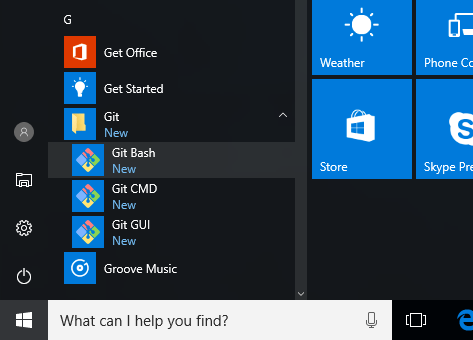
\includegraphics[width=4.5in]{images/git-bash-windows}
\end{figure}





\newpage{}
\thispagestyle {empty}

\vspace*{2cm}

\begin{figure}
		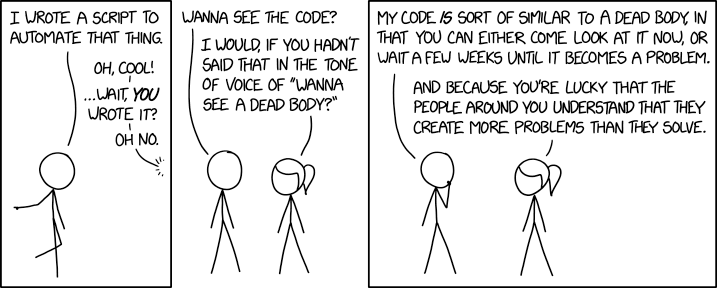
\includegraphics[width=5.5in]{images/wanna_see_the_code.png}
		\caption{This is how all of my robotics project go.}
\end{figure}

\section{How to install git}
\subsection{Command Line}
\subsection{Github Desktop App}
\subsection{Eclipse}
\subsection{Other Apps}

\section{How to use git}
\subsection{Best Practices}

\section{Fun Stuff}
\subsection{3rd Party Git Apps}



\begin{thebibliography}{9}
\bibitem{git-tower}
A large portion of this document was "liberated" from:
https://www.git-tower.com/learn/git/ebook/en/command-line/basics/why-use-version-control
\bibitem{atlassian}
https://www.atlassian.com/git/tutorials/what-is-git
\end{thebibliography}
\printindex



\end{document}
